\documentclass[a4paper, 12pt]{article}

\usepackage[T2A]{fontenc}
\usepackage[english, russian]{babel}

\usepackage{indentfirst}

% Подключим пакет, отвечающий
% за изображения
\usepackage{graphicx}

% Таким образом зададим
% название папки, где лежат картинки
\graphicspath{{./img/}}

\begin{document}
\section{Вставка картинок}
Текст текст текст и картинка: 
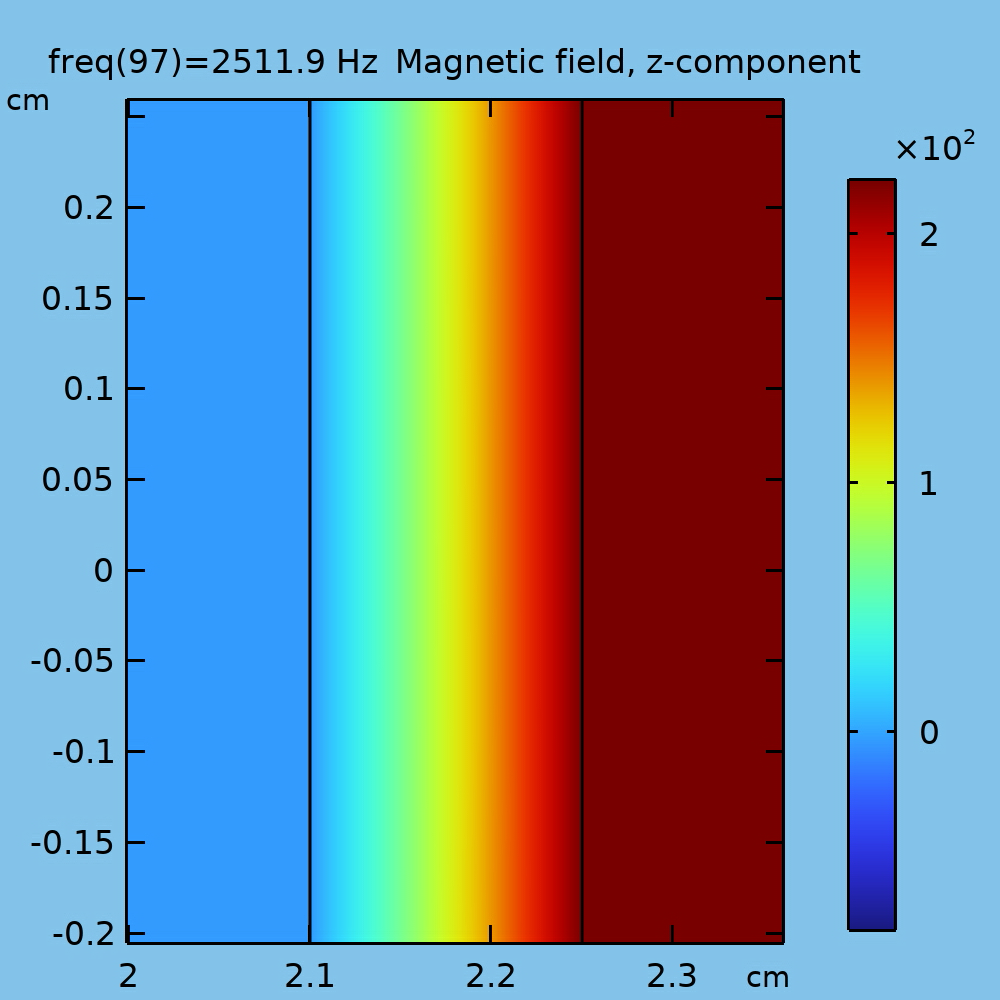
\includegraphics{09_out_img.png}. % Эта картинка лежит в одной папке с данным .tex файлом.

Перейдём на новую страницу командой <<newpage>> и попробуем ещё раз.

\newpage

Попытка 2: 
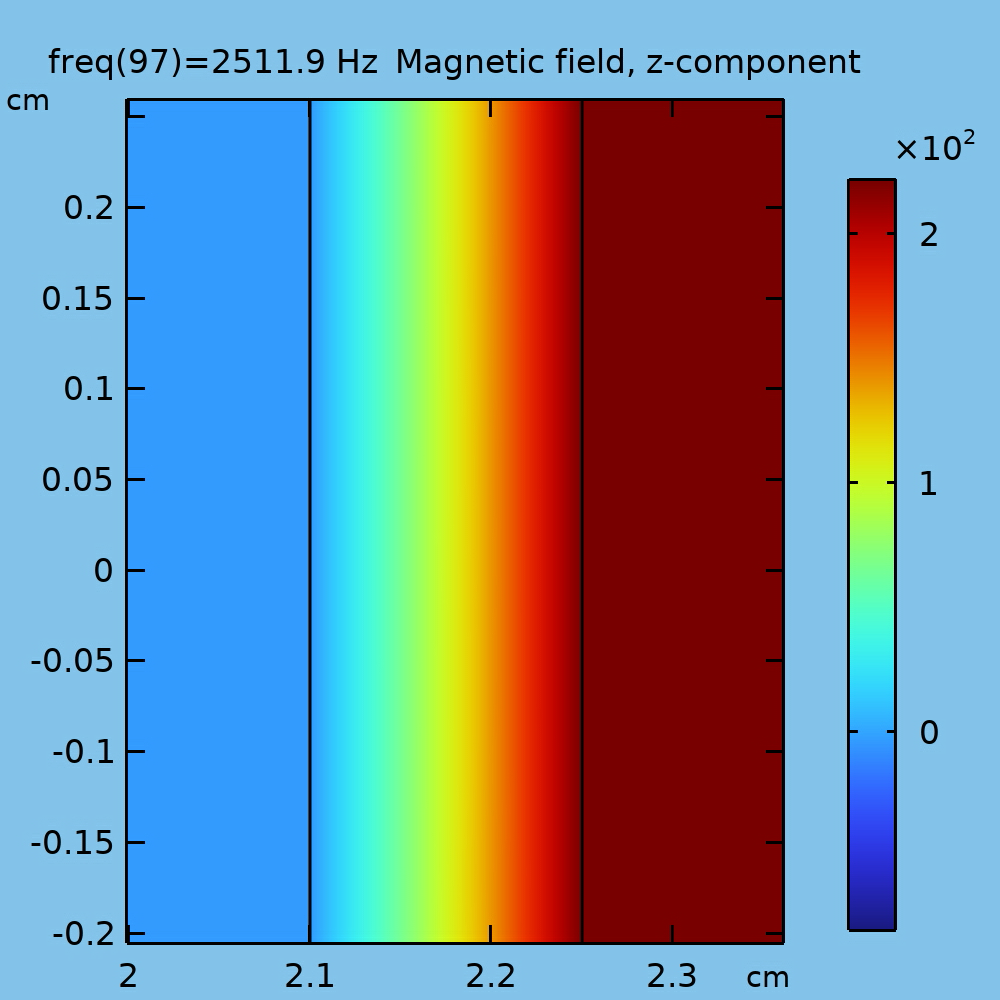
\includegraphics[scale=0.3]{09_out_img.png}

другие способы указания размера картинки:


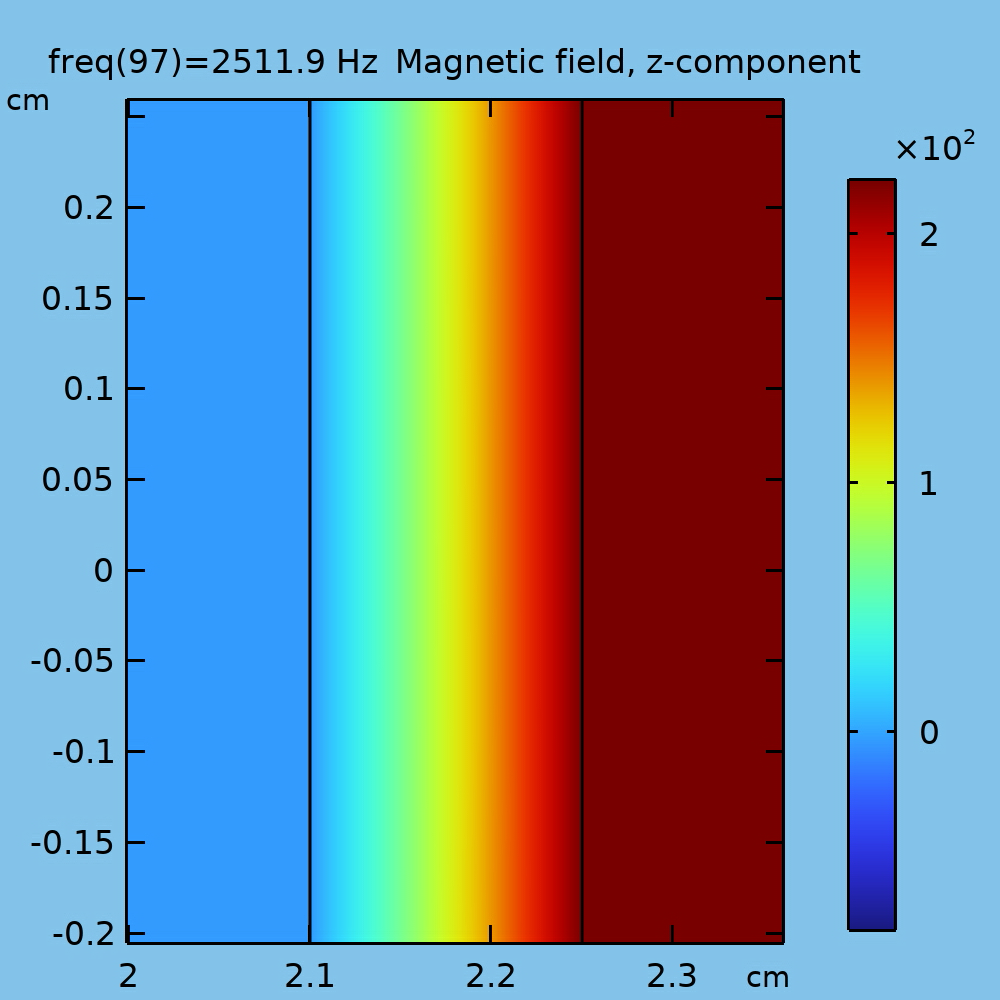
\includegraphics[width=7cm]{09_out_img.png}

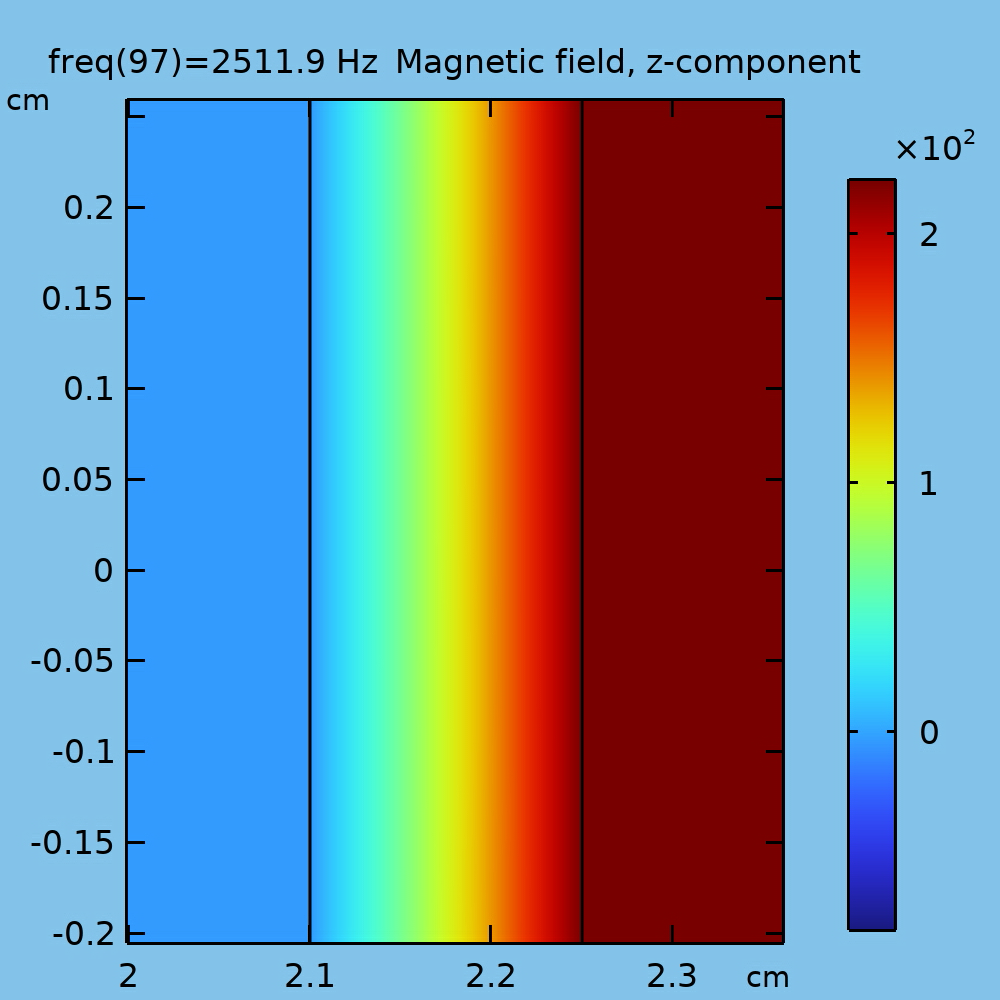
\includegraphics[height=40pt]{09_out_img.png}

В долях от ширины текста:

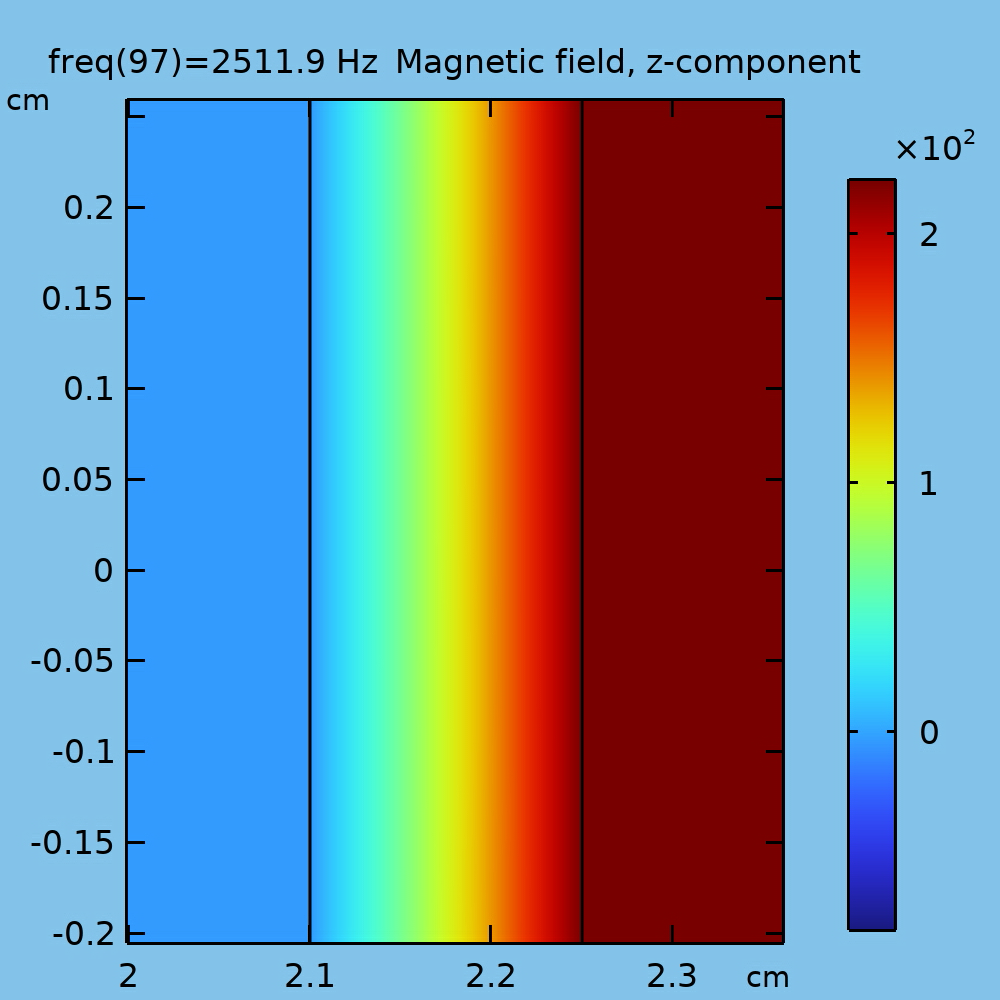
\includegraphics[width=0.5\textwidth]{09_out_img.png}

\newpage

\section{Красивый способ}
Теперь вставим рисунок \ref{fig_1} и сделаем на него ссылку, используя окружение <<figure>>:

\begin{figure}[h!] % h! -- значит, что мы хотим видеть картинку в том месте, где она находится в тексте
    \begin{center}
    		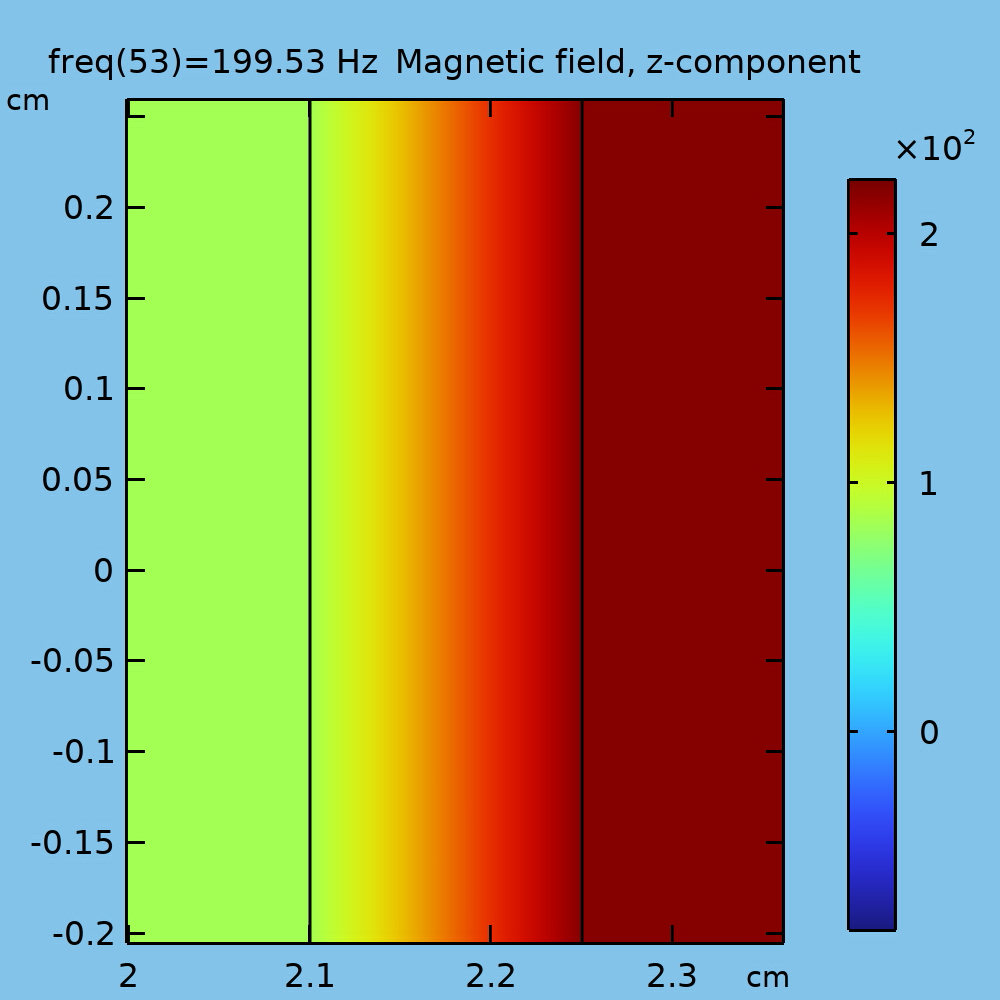
\includegraphics[width=0.85\textwidth]{in_img.png} % эта картинка -- в папке ./img
    \caption{Тут можно задать подпись рисунка}\label{fig_1}
    \end{center}
\end{figure}

\end{document}
